\documentclass[12pt, a4paper, oneside]{ctexart}
\usepackage{amsmath, amsthm, amssymb, bm, color, graphicx, geometry, mathrsfs,extarrows, braket, booktabs, array, wrapfig}
\usepackage[colorlinks,linkcolor=red,anchorcolor=blue,citecolor=blue,urlcolor=blue,menucolor=black]{hyperref}
\setCJKmainfont{方正新书宋_GBK.ttf}[ BoldFont = 方正小标宋_GBK, ItalicFont = 方正楷体_GBK]
\setmainfont{Times New Roman}  % 设置英文字体
\setsansfont{Calibri}
\setmonofont{Consolas}

\linespread{1.4}
%\geometry{left=2.54cm,right=2.54cm,top=3.18cm,bottom=3.18cm}
\geometry{left=1.84cm,right=1.84cm,top=2.18cm,bottom=2.18cm}
\newcounter{problem}  % 问题序号计数器
\newenvironment{problem}[1][]{\stepcounter{problem}\par\noindent\textbf{题目\arabic{problem}. #1}}{\smallskip\par}
\newenvironment{solution}[1][]{\par\noindent\textbf{#1解答. }}{\smallskip\par}  % 可带一个参数表示题号\begin{solution}{题号}
\newenvironment{note}{\par\noindent\textbf{注记. }}{\smallskip\par}

%%%% 图片相对路径 %%%%
\graphicspath{{figure/}} % 当前目录下的figure文件夹, {../figure/}则是父目录的figure文件夹

\everymath{\displaystyle} % 默认全部行间公式
\DeclareMathOperator*\uplim{\overline{lim}} % 定义上极限 \uplim_{}
\DeclareMathOperator*\lowlim{\underline{lim}} % 定义下极限 \lowlim_{}
\let\leq=\leqslant % 将全部leq变为leqslant
\let\geq=\geqslant % geq同理

%%%% 一些宏定义 %%%%
\def\bd{\boldsymbol}        % 加粗(向量) boldsymbol
\def\disp{\displaystyle}    % 使用行间公式 displaystyle(默认)
\def\tsty{\textstyle}       % 使用行内公式 textstyle
\def\sign{\text{sign}}      % sign function
\def\wtd{\widetilde}        % 宽波浪线 widetilde
\def\R{\mathbb{R}}          % Real number
\def\N{\mathbb{N}}          % Natural number
\def\Z{\mathbb{Z}}          % Integer number
\def\Q{\mathbb{Q}}          % Rational number
\def\C{\mathbb{C}}          % Complex number
\def\K{\mathbb{K}}          % Number Field
\def\P{\mathbb{P}}          % Polynomial
\def\d{\mathrm{d}}          % differential operator
\def\e{\mathrm{e}}          % Euler's number
\def\i{\mathrm{i}}          % imaginary number
\def\re{\mathrm{Re}}        % Real part
\def\im{\mathrm{Im}}        % Imaginary part
\def\res{\mathrm{Res}}      % Residue
\def\ker{\mathrm{Ker}}      % Kernel
\def\L{\mathcal{L}}         % Loss function
\def\wdh{\widehat}          % 宽帽子 widehat
\def\ol{\overline}          % 上横线 overline
\def\ul{\underline}         % 下横线 underline
\def\add{\vspace{1ex}}      % 增加行间距
\def\del{\vspace{-1.5ex}}   % 减少行间距

%%%% 定理类环境的定义 %%%%
\newtheorem{theorem}{定理}

%%%% 基本信息 %%%%
\newcommand{\RQ}{\today} % 日期
\newcommand{\km}{泛函分析} % 科目
\newcommand{\bj}{强基数学002} % 班级
\newcommand{\xm}{吴天阳} % 姓名
\newcommand{\xh}{2204210460} % 学号

\begin{document}

%\pagestyle{empty}
\pagestyle{plain}
\vspace*{-15ex}
\centerline{\begin{tabular}{*5{c}}
    \parbox[t]{0.25\linewidth}{\begin{center}\textbf{日期}\\ \large \textcolor{blue}{\RQ}\end{center}} 
    & \parbox[t]{0.2\linewidth}{\begin{center}\textbf{科目}\\ \large \textcolor{blue}{\km}\end{center}}
    & \parbox[t]{0.2\linewidth}{\begin{center}\textbf{班级}\\ \large \textcolor{blue}{\bj}\end{center}}
    & \parbox[t]{0.1\linewidth}{\begin{center}\textbf{姓名}\\ \large \textcolor{blue}{\xm}\end{center}}
    & \parbox[t]{0.15\linewidth}{\begin{center}\textbf{学号}\\ \large \textcolor{blue}{\xh}\end{center}} \\ \hline
\end{tabular}}
\begin{center}
    \zihao{-3}\textbf{第七次作业}
\end{center}
\vspace{-0.2cm}
% 正文部分
\begin{problem}[(2.1.2)]
    设$A\in L(X,Y)$,求证:
    \begin{equation*}
        \text{(1). }||A||=\sup_{||x||\leq 1}||Ax||;\quad \text{(2). }||A||=\sup_{||x||<1}||A||.
    \end{equation*}\del\del\del
\end{problem}
\begin{proof}
    (1). 当$|x| < 1$时,$||Ax||\leq ||A||\cdot ||x|| < ||A||$,则$||A|| = \sup_{||x||\leq 1}||Ax||$.

    (2). 由上确界定义可知$\forall \varepsilon > 0$,$\exists ||x_0||=1$使得$||Ax_0|| > ||A||(1-\varepsilon)$,令$x_n = x_0\left(1-\frac{1}{n}\right)$,则$||x_n|| = \left(1-\frac{1}{n}\right)||x_0|| < 1$且$x_n\to x_0$,又由于$A$有界$||A|| < \infty$,则
    \begin{equation*}
        ||Ax_n|| = ||Ax_n-Ax_0+Ax_0||\leq||A||\cdot||x_n-x_0|| + ||Ax_0||\to||A||(1-\varepsilon),\ (n\to\infty)
    \end{equation*}
    由$\varepsilon$的任意性可知$\sup_{||x|| < 1}||Ax|| = ||A||$.
\end{proof}
\begin{problem}[(2.1.3)]
    设$f\in L(X,\R)$,求证:
    \begin{equation*}
        \text{(1). }||f||=\sup_{||x||=1}f(x);\quad \text{(2). }\sup_{||x||<\delta}f(x)=\delta||f||,\ (\forall \delta > 0).
    \end{equation*}\del\del\del
\end{problem}
\begin{proof}
    (1). 由于$f(-x) = -f(x)$,则$\forall \varepsilon > 0$使得$|f(x_0) > ||f||-\varepsilon$.

    若$f(x_0) < 0$,则$\exists ||-x_0|| = 1$使得$f(-x_0) = -f(x_0) = |f(x_0)| > ||f||-\varepsilon$.

    若$f(x_0)\geq 0$,则$f(x_0) = |f(x_0)| > ||f||-\varepsilon$.

    综上,$\exists ||x_1|| = 1$使得$f(x_1) > ||f||- \varepsilon$,则$||f|| = \sup_{||x||=1}f(x)$.

    (2). 由上题可知$||f||=\sup_{||x|| < 1}f(x)$,$\forall \varepsilon > 0$,$\exists ||x_0|| < 1$,使得
    \begin{equation*}
        f(x_0) > ||f|| - \varepsilon\Rightarrow f(\delta x_0) > \delta ||f|| - \delta \varepsilon,\ (\forall \delta > 0)
    \end{equation*}
    则$\exists y_0 = \delta x_0\in B(\delta)$使得$f(y_0)>\delta ||f||-\delta \varepsilon$,则$\sup_{||y||<\delta}f(y) = \delta||f||$.
\end{proof}
\begin{problem}[(2.1.4)]
    设$y(t)\in C[0,1]$,定义$C[0,1]$上的泛函$f(x) = \int_0^1x(t)y(t)\,\d t,\ (\forall x\in C[0,1])$,求$||f||$.
\end{problem}
\begin{solution}
    由于
    \begin{equation*}
        |f(x)| = \left|\int_0^1x(t)y(t)\,\d t\right|\leq \int_0^1|x(t)|\,\d t\int_0^1|y(t)|\,\d t\leq \max_{t\in[0,1]}\{x(t)\}\int_0^1|y(t)|\,\d t
    \end{equation*}
    则$||f||\leq \int_0^1|y(t)|\,\d t$. 下证$||f||\geq \int_0^1|y(t)|\,\d t$.

    由于$y$连续,则$\forall \varepsilon > 0$,$n\in \N$使得$\forall |x_1-x_2|\leq 1/n$,有$|y(x_1)-y(x_2)| < \varepsilon$,构造$[0,1]$上的$n$等分区间$\pi : 0=a_0 < a_1<\cdots <a_n=1$,其中$a_i-a_{i-1}=1/n\ (i=1,2,\cdots,n)$. 令
    \begin{equation*}
        \begin{aligned}
            A=&\ \bigcup\{[a_{i-1},a_i]:\forall t\in [a_{i-1},a_i],y(t)\neq 0\},\\
            B=&\ \bigcup\{[a_{i-1},a_i]:\exists t_0\in [a_{i-1}, a_i],y(t)=0\}.
        \end{aligned}\quad 
        \tilde{x}=\begin{cases}
            \text{sgn}(y(t)),&\quad t\in A,\\
            \text{线性函数},&\quad t\in B.
        \end{cases}
    \end{equation*}
    \clearpage
    \ \del\del
    \begin{align*}
        f(\tilde{x}) =&\ \int_0^1\tilde{x}(t)y(t)\,\d t = \int_A|y|\,\d t+\int_B\tilde{x}(t)y(t)\,\d t\\
        \geq&\ \int_A|y|\,\d t-\int_B|y|\,\d t = \int_0^1|y|\,\d t-2\int_B|y|\,\d t > \int_0^1|y|\,\d t-2\varepsilon
    \end{align*}
    由于$||\tilde{x}||\leq 1$则
    \begin{equation*}
        \int_0^1|y|\,\d t-2\varepsilon < f(\tilde{x})\leq ||f||\cdot||x||\leq ||f||\leq \int_0^1|y|\,\d t
    \end{equation*}
    由$\varepsilon$的任意性可知$||f|| = \int_0^1|y|\,\d t$.
\end{solution}
\begin{problem}[(2.1.5)]
    设$f$是$X$上的非零有界线性泛函,令$d=\inf\{||x||:f(x)=1,x\in X\}$,求证$||f|| = 1/d$.
\end{problem}
\begin{proof}
    $\forall \varepsilon > 0$,$\exists x_0\in X$,$f(x_0) = 1$,使得
    \begin{equation*}
     ||x_0|| < d(1+\varepsilon)\Rightarrow \frac{1}{d}\cdot\frac{1}{1-\varepsilon}<\frac{1}{||x_0||}=\frac{f(x_0)}{||x_0||}=f\left(\frac{x_0}{||x_0||}\right)
    \end{equation*}
    则$1/d = \sup_{||x||=1}f(x) = ||f||$.
\end{proof}
\begin{problem}[(2.1.6)]
    设$f\in X^*$,求证:$\forall \varepsilon >0$,$\exists x_0\in X$,使得$f(x_0) = ||f||$,且$||x_0|| < 1+\varepsilon$.
\end{problem}
\begin{proof}
    不妨令$||f||\neq 0$,则$\forall \varepsilon > 0$,$\exists x_1\in X$,且$||x_1||\neq 0$,使得
    \begin{equation*}
        f\left(\frac{x_1}{||x_1||}\right) > \frac{||f||}{1+\varepsilon}\Rightarrow \frac{||x_1||}{f(x_1)}||f|| < 1+\varepsilon
    \end{equation*}
    令$x_0 = \frac{x_1}{f(x_1)}||f||$,则$||x_0|| < 1+\varepsilon$,且$f(x_0) = ||f||$.
\end{proof}
\begin{problem}[(2.1.7)]
    设$T:X\to Y$是线性的,令$N(T):=\{x\in X:Tx=\theta\}$.

    (1). 若$T\in L(X,Y)$,求证:$N(T)$是$X$的闭线性子空间.

    (2). 问$N(T)$是$X$的闭线性子空间能否推出$T\in L(X,Y)$?

    (3). 若$f$是线性泛函,求证:$f\in X^*\iff N(f)\text{是闭线性子空间.}$
\end{problem}
\begin{proof}
    (1). $\forall \{x_n\}\subset N(T)$收敛于$x$,则$0=Tx_n\to Tx$,则$x\in N(T)$.

    (2). 反例:在$l^{\infty} = \left\{x=(\xi_1,\xi_2,\cdots):\sum_{i=1}^\infty|x_i| < \infty\right\}$中,范数为$||x|| = \sup_{n\geq 1}|\xi_n|$,$a=\{1,-1,0,\cdots\}$,构造$f(x) = \sum_{i=1}^\infty \xi_i,\ (\forall x=(\xi_1,\xi_2,\cdots))$,则$f$是$l^{\infty}$上的线性泛函. 令$Tx = x-af(x)$,则$x-af(x) = \theta\Rightarrow a = \frac{x}{f(x)}\Rightarrow ||a|| = f(x) - f(a)f(x) = \theta$,则$N(T) = \{\theta\}$.

    假设$T$有界,$\exists M$使得
    \begin{align*}
        &\ ||Tx||\leq M||x||\Rightarrow ||x-af(x)||\leq M||x||\Rightarrow ||af(x)||-||x||\leq M||x||\\
        \Rightarrow&\ ||a||\cdot |f(x)|\leq (M+1)||x||\Rightarrow |f(x)|\leq (M+1)||x||
    \end{align*}
    则$f$有界. 下证$f$无界.

    令$a_n = \{\underbrace{1,\cdots,1}_{n\text{个}},0,\cdots\}$则$||a_n|| = 1,\ f(a_n) = n$,而$\frac{||f(a_n)||}{||a_n||} = n\to\infty,\ (n\to\infty)$,所以$f$无界. 故$T$无界.

    (3). 充分性:由(1)可得.

    必要性:反设$f$在单位球面上无界,则$\forall n\in \N$,$\exists x_n\in X$且$||x_n|| = 1$,$f(x_n) \geq n\Rightarrow \frac{1}{n}\geq \frac{1}{f(x_n)}$,令$y_n = \frac{x_n}{f(x_n)} - \frac{x_1}{f(x_1)}$,则
    \begin{equation*}
        \left|\left|y_n+\frac{x_1}{f(x_1)}\right|\right| = \left|\left|\frac{x_n}{f_n}\right|\right| = \frac{1}{f(x_n)}\leq \frac{1}{n}\to 0\quad(n\to\infty)
    \end{equation*}
    则$y_n\to-\frac{x_n}{f(x_1)}$,且$f(y_n) = 0$,则$\{y_n\}\subset \ker f$收敛,但是$f(-\frac{x_1}{f(x_1)}) = -1\neq 0$,则$-\frac{x_1}{f(x_1)}\notin \ker f$与$\ker f$是闭的矛盾. 故$f$在单位球面上有界,则$f\in X^*$.
\end{proof}

% 下面给一些功能的写法
\iffalse
% 图片模板
\centerline{
    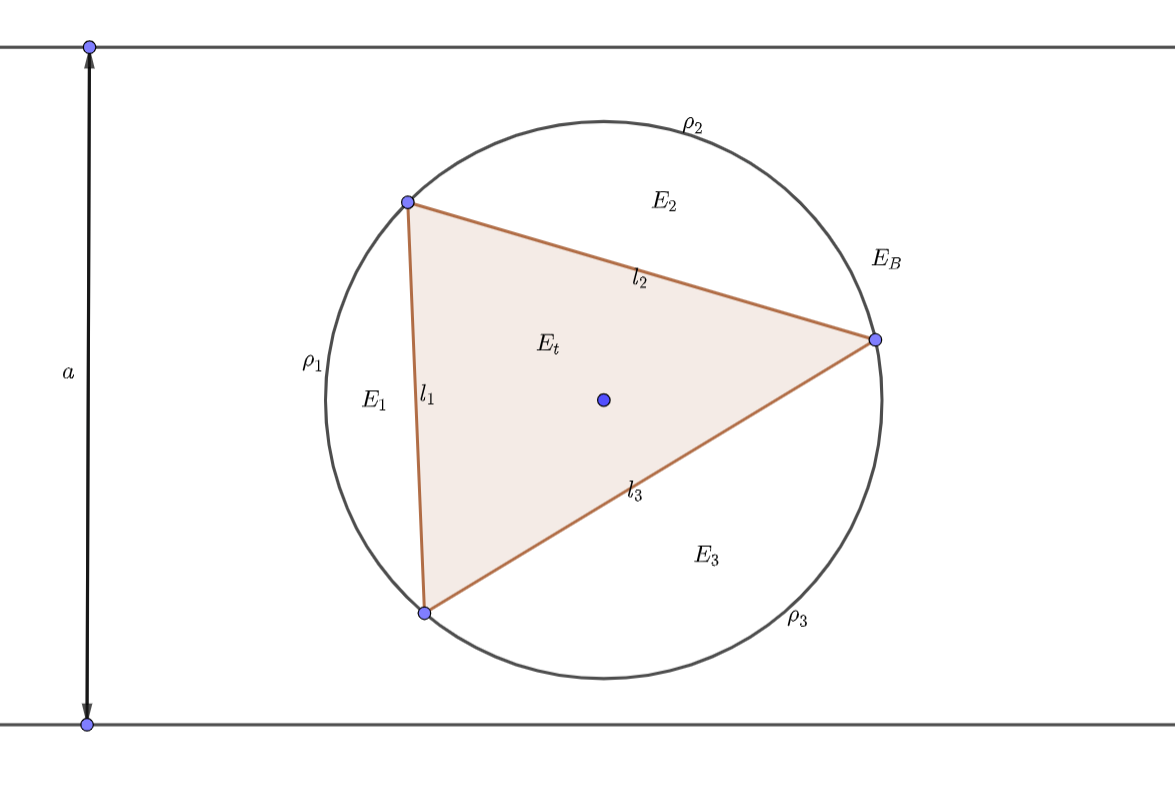
\includegraphics[width=0.8\textwidth]{figure.png}
}
% 表格模板
\renewcommand\arraystretch{0.8} % 设置表格高度为原来的0.8倍
\begin{table}[!htbp] % table标准
    \centering % 表格居中
    \begin{tabular}{p{1cm}<{\centering}p{1cm}<{\centering}p{3cm}<{\centering}p{5cm}<{\centering}} % 设置表格宽度
    %\begin{tabular}{cccc}
        \toprule
        $x_i$ & $f[x_1]$ & $f[x_i,x_{i+1}]$ & $f[x_i,x_{i+1},x_{i+2}]$ \\
        \midrule
        $x_0$ & $f(x_0)$ &                  &                          \\
        $x_0$ & $f(x_0)$ & $f'(x_0)$        &                          \\
        $x_0$ & $f(x_1)$ & $\frac{f(x_1)-f(x_0)}{x_1-x_0}$ & $\frac{f(x_1)-f(x_0)}{(x_1-x_0)^2}-\frac{f'(x_0)}{x_1-x_0}$\\
        \bottomrule
    \end{tabular}
\end{table}

\def\Log{\text{Log}} % 一个简单的宏定义
$\Log$ % 调用方法
\fi

\end{document}